\documentclass[resume]{subfiles}


\begin{document}
\begin{multicols}{3}
\section{Opamp 1}


\subsection{Catégories d'AOP idéaux}
\begin{figure}[H]
    \centering
    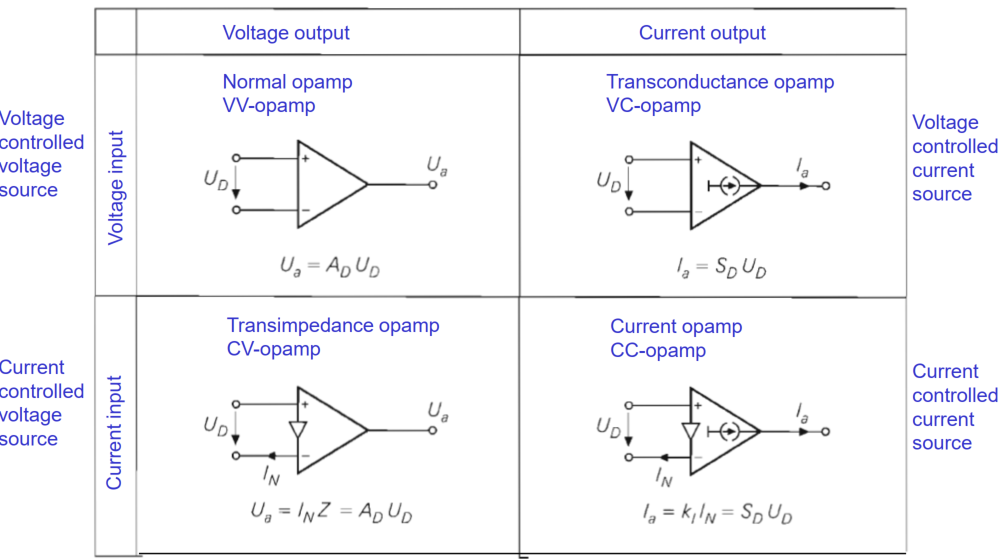
\includegraphics[width=\columnwidth]{../images/OpAmp1/categoriesAOP.png}
\end{figure}
\paragraph{Amplificateur de tension} Entrée en tension, sortie en tension
$$U_a=A_DU_D$$
\paragraph{Amplificateur à transconductance} Entrée en tension, sortie en courant
$$I_a=S_DU_D$$
\paragraph{Amplificateur à transimpédance} Entrée en courant, sortie en tension 
$$U_a=I_NZ=A_DU_D$$
\paragraph{Amplificateur de courant} Entrée en courant, sortie en courant
$$I_a=k_II_N=S_DU_D$$
\subsection{Caractéristique de transfert}
\begin{figure}[H]
    \centering
    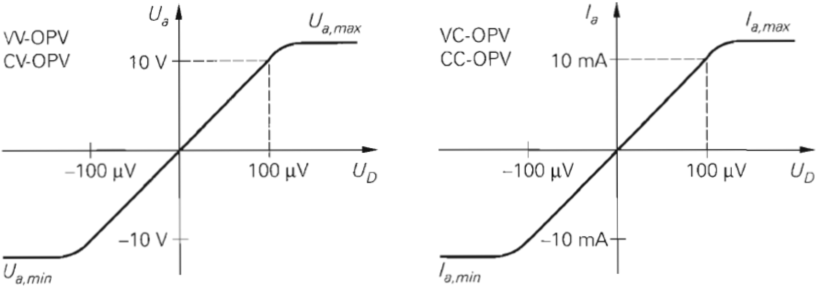
\includegraphics[width=0.8\columnwidth]{../images/OpAmp1/carTransAOP.png}
\end{figure}
\begin{itemize}
\item gain idéal infini
\item $U_{out}$ limité aux tensions d'alimentation
\end{itemize}

\subsection{Control loop diagram}
\begin{figure}[H]
    \centering
    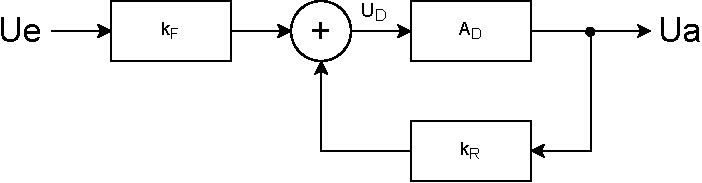
\includegraphics[width=0.8\columnwidth, page=1]{Schemas-crop.pdf}
\end{figure}

\begin{itemize}
\item $U_D = k_FU_e - k_RU_a$
\item $A = \frac{U_a}{U_e} = \frac{k_FA_D}{1+k_RA_D} \cong \frac{k_F}{k_R}$ (pour $A_D$ grand) 
\end{itemize}

\subsubsection{non-inverseur}
\begin{itemize}
\item $k_F = 1$
\item $k_R = \frac{R_1}{R_1+R_N}$
\item $A = 1+\frac{R_N}{R_1}$
\end{itemize}
$R_N$ est la résistance de contre réaction et $R_1$ la résistance mise à la masse.

\subsubsection{inverseur}
\begin{itemize}
\item $k_F = \frac{-R_N}{R_1+R_N}$
\item $k_R = \frac{R_1}{R_1+R_N}$
\item $A_D = \frac{U_a}{k_FU_e-k_RU_a}$
\item $A = k_F\frac{A_D}{1+k_RA_D}$
\end{itemize}

\subsubsection{différentiel}
\begin{itemize}
\item $k_F = \frac{R_1}{R_1+R_2}$
\item $k_R = \frac{R_2}{R_1+R_2}$
\item $A = \frac{R_1A_D}{R_1+R_2+R_2A_D} \cong \frac{R_1}{R_2}$ (pour $A_D$ grand)
\end{itemize}
$R_1$ contre réaction et résistance à la masse / $R_2$ résistance d'entrée (+ et -)

\subsection{Montage interne AOP}
\subsubsection{Amplificateur différentiel}
\begin{figure}[H]
    \centering
    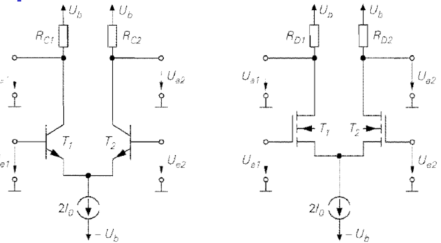
\includegraphics[width=0.8\columnwidth]{../images/OpAmp1/m_diff.png}
\end{figure}
\paragraph{Pour les petits signaux}
\begin{figure}[H]
    \centering
    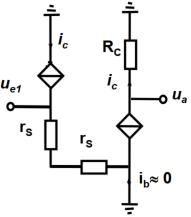
\includegraphics[width=0.5\columnwidth]{../images/OpAmp1/mPS_diff.png}
\end{figure}
\begin{itemize}
\item $A_1 = \frac{R_c}{2r_s}$
\item $A_2 = \frac{-R_c}{2r_s}$
\end{itemize}

\subsubsection{Miroir de courant}
\begin{figure}[H]
    \centering
    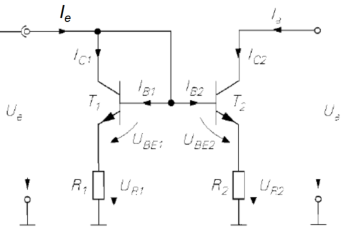
\includegraphics[width=0.6\columnwidth]{../images/OpAmp1/m_mirroir.png}
\end{figure}
Facteur de translation de courant $k = \frac{R_1}{R_2}$
\begin{figure}[H]
    \centering
    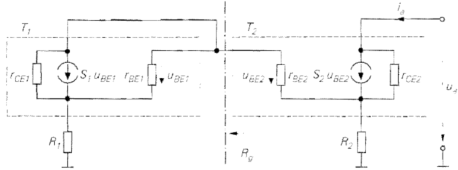
\includegraphics[width=0.9\columnwidth]{../images/OpAmp1/mPS_mirroir.png}
\end{figure}

\subsubsection{Charge active}
On utilise un miroir de courant comme charge active.
\begin{figure}[H]
    \centering
    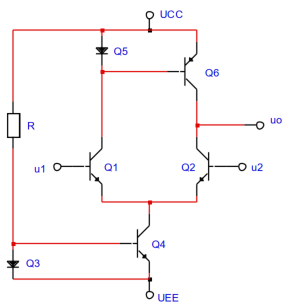
\includegraphics[width=0.5\columnwidth]{../images/OpAmp1/m_chrgact.png}
\end{figure}

\subsubsection{Cascode}

\subsubsection{Conversion d'impédance}

\subsubsection{Push-Pull}

\subsubsection{Darlington}

\end{multicols}
\end{document}